\begin{itemize}
    \item Two questions, each question carries 15 points.
    \item These are essay-type questions that may not have a single answer. I will grade based on the correctness and the relevancy of your answer, and whether your idea is clearly explained. You are welcome to include figures or formula to aid your answer.
\end{itemize}

\newpage
\begin{homeworkProblem}
    Please read the following article:

    \noindent\textbf{Unraveling the dynamics of conductive filament in MoS$_2$-based memristors by operando transmission electron microscopy, Nature Communications 16, 7433 (2025)} \url{https://doi.org/10.1038/s41467-025-62592-2}

    In this article, two imaging methods in TEM were used to probe the Ag filament formation in MoS$_2$ memristor: high-angle annular dark-field (HAADF) and energy-dispersive X-ray spectroscopy (EDXS) elemental mapping.
    \begin{enumerate}[a)]
        \item From what you learnt from the class, explain the operation principles of these two imaging mechanisms. How they can be used to image the Ag filament in MoS$_2$ in the work presented in the above paper. \textbf{(8 points)}
            \begin{callout}{Solution:}

                \begin{multicols}{2}
                
                The first of the two techniques, high-angle annular dark-field (HAADF), is one detector mode for STEM, with the other two being annular dark-field and bright-field. Each mode differs in the angle of collected electrons. For HAADF, electrons are collected at the highest angle (shown in figure \ref{fig:stem-tem_detector_modes}), as the name suggests. The exact angle can vary depending on author, but it's often >50 mrads or >$4^{\circ}$ off-axis. Electrons which scatter this way are incoherent (aka Rutherford scattered, or elastically scattered) and highly sensitive to atomic number.

\begin{figure}[H]
  \centering
  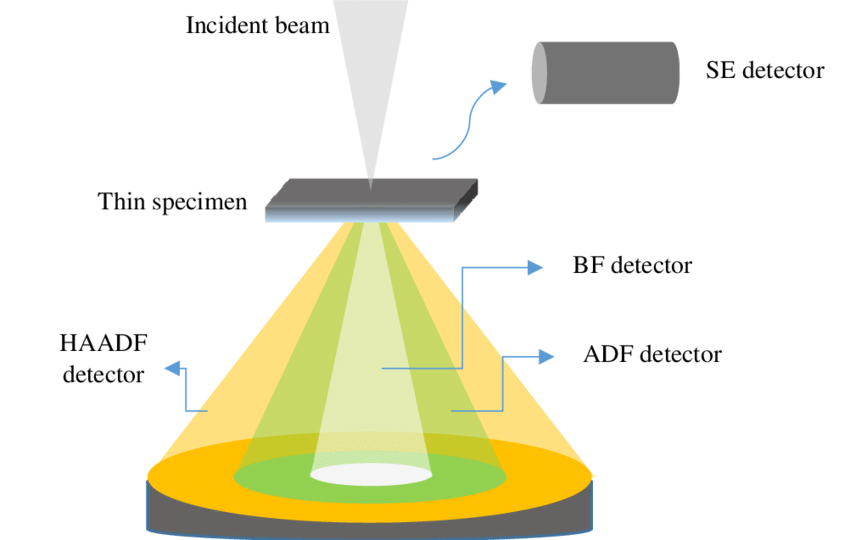
\includegraphics[width=0.45\textwidth]{../assets/fig:STEM-TEM_detector_modes.png}
  \caption{Schematic of the HAADF, conventional annular dark-field (ADF) and BF detectors in a TEM. \cite{AbouSaleh2020}}
  \label{fig:stem-tem_detector_modes}
\end{figure}

                The second of the two techniques, energy-dispersive x-ray spectroscopy (EDXS) utilizes x-rays generated by excitations in the scattering process to identify chemical composition. The process has two parts: x-ray generation and x-ray measurement. When an electron diffracts off of an atom, an electron may be replaced by the incoming high-energy electron, producing a hole simultaneously. The amount by which the energy is raised can be complicated to model, but depends on Z. A few things can happen in this process:
                \begin{enumerate}[1.]
                    \item The high-energy electron drops to a lower shell, emitting a photon in the x-ray band
                    \item The vacancy is filled, but the excess energy is transferred to another electron which ejects it.
                \end{enumerate}

                EDXS relies on the first case. X-rays can be collected using a counter above the sample. Since each element has a distinct x-ray spectra, each may be identified by the collected signature.
                \end{multicols}

                In the article, the authors collect both a HAADF image of the cross-section and setup inside the STEM, as well as a composite map for their sample using EDXS. This is used to justify that they actually observe what they claim, as it is easy to distinguish the filament forming between the MoS$_2$ layers, (their 2nd figure). The high Z-contrast and elemenatal mapping via EDXS is useful in identifying the Ag filament form, and quantitatively elaborate on contrast as it relates to electronic state.

            \end{callout}

        \item Was the work presented in the above paper done in a conventional TEM or a scanning TEM (STEM)? In addition to simply finding your answer from the method section, I expect you to explain why the presented measurement can only be done with this specific type of TEM (but not the other type). \textbf{(2 points)}
            \begin{callout}{Solution:}

            All work was done using a STEM. First, a tighly focused beam is required to produce a HAADF image. A collimated TEM uses an aperture to collect scattered electrons, whereas a STEM focuses its beam to a very small point and uses annular detectors to collect a dark-field image. HAADF is simply the image formed by the high angle annular detector.

            Second, EDXS also can only be done (effectively) with STEM, since the signal is integrated over the area which electrons "illuminate" the sample. For a collimated TEM the signature is indecipherable because the illuminated area is typically the entire sample. For a STEM though, it is possible to determine elemental signatures with high spatial resolution, as the beam is focused to a small point.

            \end{callout}
        \item Please provide pros and cons for the HAADF and EDXS method when they were used for the measurements presented in the paper. \textbf{(2 points)}
            \begin{callout}{Solution:}

                The main advantage of using HAADF and EDXS for this paper is the high spatial resolution, \textit{in real space} which is required - it would be very difficult to image the interface without doing so in real space. EDXS and the high Z-contrast of HAADF are essential for observing the structural changes throughout the device, since it would be difficult to justify that there is or is not a wire forming without the elemental mapping and high-contrast image. Specifically, EDXS is a good supplement to HAADF, since it provides quantitative mapping of elements as opposed to contrast clues. HAADF is also ideal for use  in smaller samples (as in this paper), as inelastic scattering events occur more easily in thicker samples.

                In terms of limitations, STEM tends to have less signal than a collimated TEM (and can therefore have reduced contrast). This is because a small collection angle is needed to account for the large divergence of the beam. Of course, HAADF uses larger collection angles, so this may be negligable. Additionally, EDXF may require long acquisition times, and this paper is trying to image devices which change under bias in the duration of seconds which makes this experiment challenging.

                It is slightly tangential, but I find it interesting that EDXS has limitations in the elements which can be resolved: hydrogen, helium, lithium, beryllium, up to atomic number 5, do not have electrons in outer orbitals which can be replaced and thus cannot be measured \cite{enwiki:1320764489}. 
            \end{callout}
        \item Explain what information does Fig.\ 3 (a and b) tell us regarding the filament formation process. \textbf{(3 points)}
            \begin{callout}{Solution:}

            Their third figure images the set-reset behavior during one full cycle of the memristor with a large field-of-view (FOV) such that it is possible to observe the full device. The process shows that the Ag particle shrinks while the filament forms during intercalation, and that this also introduces deformations to the MoS$_2$ layers which persist after deintercalation. It is also observed that there can be some Ag left in the bundle after reset. At the same time, this is mapped to bias, such that these structural changes can be comapred to the electronic state of the device.

            \end{callout}
    \end{enumerate}
\end{homeworkProblem}

\newpage
\begin{homeworkProblem}
    Please read the following article:

    
    \noindent\textbf{Revealing interfacial failure mechanism of silicon based all solid state batteries via cryogenic electron microscopy, Nature Communications 16, 9731 (2025)} \url{https://doi.org/10.1038/s41467-025-64697-0}

    

    \begin{enumerate}[a)]

        \item In this work, the authors used cryo-FIB and cryo-TEM/STEM for sample preparation and characterization, respectively. Provide the reasons why an extremely low temperature is needed for all these processes. \textbf{(1 point)}

            \begin{callout}{Solution:}

                Cryo-TEM/STEM was used to image the two interfacial structures: the nanocrystalline $\mathrm{Li_2S}$ dispersed in an amorphous matrix, and $\mathrm{Li_2S}$ nanocrystals in the $\mathrm{Li_{10}GeP_{2}S_{12}}$ (LGPS) substrate. As this is essentially the characterization of the internal structure of the battery. To do so, Extremely cold, vacuum conditions are required in order to avoid changes in the chemistry/structure due to chemical reactions.

            \end{callout}

        \item The authors used a number of characterization techniques to study the reaction of the solid state electrolyte, e.g., the LGPS in Fig.\ 2, with the Li. In figure 2, results from the following characterization techniques are presented:

            \begin{itemize}
                \item Fig.\ 2a\&b: cross-sectional SEM with central backscattered electron (CBS) images and EDS mapping.
                \item Fig.\ 2c-e: X-ray photoemission spectroscopy (XPS)
                \item Fig.\ 2f-h: STEM images with mapping from electron energy loss spectroscopy (EELS).
            \end{itemize}

            Discuss and explain what information are provided from each of the above characterization method on the reaction of the LGPS with the Li. \textbf{(7 points)}

            \begin{callout}{Solution:}

                \subsubsection{Fig. 2a\&b: cross-sectional SEM with central backscattered electron (CBS) images and EDS mapping.}

                Fundamentally, a cross-sectional, real-space image (Fig. 2a) is required to look at the interfaces in the battery. The central backscattered electron (CBS) image does this with higher Z-contrast (as the backscattering process is highly dependent on Z). 

                To determine which layer is which, and guarantee that there is really an interface, EDS mapping can characterize the composition. The authors use a line cut to show there are indeed composition changes, and what elements they consist of (Fig. 2b).

                \subsubsection{Fig. 2c-e: X-ray photoemission spectroscopy (XPS)}

                Fig. 2c-e show there are additional peaks in the XPS spectrum after cycling 100 times, and this contributes to the argument that there are new chemical species (namely, they can tell which ones by the peaks) appearing during cycling.

                \subsubsection{Fig. 2f-h: STEM images with mapping from electron energy loss spectroscopy (EELS).} 

                The authors use scanning transmission electron microscopy (STEM) \& electron energy loss spectroscopy (EELS) are used for structural analysis of the interfacial reaction layer (IRL). Fig. 2f shows the STEM image and elemental mapping and confirms there is a decomposition into $\mathrm{Li_2S}$ and LGPS in this layer. This supports the theory the authors present that these products contribute to the loss of active Lithium in the battery, and therefore lower capacity.

            \end{callout}

        \item With all the information provided from Fig.\ 2, provide a possible explanation on why the IRL and IRR phases appear to be darker than the more pristine LGPS phase in the SEM image (Fig.\ 2a). \textbf{(2 points)}

            \begin{callout}{Solution:}

                The IRL and IRR were proven to be sites at which there is the decomposition of pristine products to form LGPS \& $\mathrm{Li_2S}$. $\mathrm{Li_2S}$ has a lower average Z than LGPS, and because of the sensitivity towards Z afforded by CBS (higher Z results in reduced backscattering), we expect a contrast shift due to the appearance of these products in these regions.

            \end{callout}

        \item Comparing the results from LGPS (Fig.\ 2) and LSPSC (Fig.\ 4) solid-state electrolytes, what is the major difference on the reaction of the electrolyte with Li between the two material systems? Support your answers with the experimental results presented in those two figures. \textbf{(3 points)}

            \begin{callout}{Solution:}
            
                For the LGPS electrolyte, the authors explained their findings as a continuous decomposition of the electrolyte due to reaction with Li; however, with LSPSC this is clearly not the case since the interfacial layer shown in their SEM image is instead very thin. The XPS characterization of the interface is also different, in that there is $\mathrm{Li_2S}$ formation, but the P and Cl peaks are unchanged. Clearly, $\mathrm{Li_2S}$ is forming, but there are fewer decomposition products. How this process saturates I talk about in the next section.

            \end{callout}

        \item How the difference you described in part (d) related to the very different capacity loss for the two batteries (see Fig.\ 1a for the capacity loss)? \textbf{(2 points)}

            \begin{callout}{Solution:}

            The authors note that electrically,$\mathrm{Li_2S}$ is insulating, but an ionic conductor. The formation of this thin, dense layer in LSPSC, as opposed to needles in LGPS, appears to block the degredation of the device by suppressing further reactions after its formation.

            \end{callout}

    \end{enumerate}

\end{homeworkProblem}

\newpage
\bibliography{./_citations.bib}% Produces the bibliography via BibTeX.
